\chapter{Distribuição de Chaves}
\label{cha:distribuicao-chaves}

Até agora, todos os sistemas criptográficos que discutimos são {\em simétricos}.
Isso significa que as partes envolvidas na comunicação compartilham uma mesma informação secreta, que chamamos de {\em chave}.
Já falamos sobre como gerar essas chaves, mas ainda não abordamos uma questão fundamental em criptografia:
{\em como distribuir essas chaves} de forma segura entre as partes.

Nesta seção, vamos explorar dois métodos distintos para resolver o problema da distribuição de chaves.
O primeiro método envolve a existência de uma {\em autoridade central} responsável por distribuir as chaves para as partes interessadas.
Essa abordagem é direta, mas depende fortemente da confiança na autoridade central.

O segundo método nos introduz a um novo paradigma chamado {\em criptografia assimétrica}.
Ao contrário da criptografia simétrica, onde a mesma chave é usada para criptografar e descriptografar, na criptografia assimétrica cada parte tem um par de chaves:
uma pública e outra privada.
Esse conceito será explorado mais detalhadamente nos próximos dois capítulos, onde veremos como a criptografia assimétrica resolve o problema de distribuição de chaves de forma elegante e segura.

\section{Centro de Distribuição de Chaves}
\label{sec:kdc}

No modelo de {\em Centro de Distribuição de Chaves} (KDC), a segurança das comunicações entre os usuários é centralizada em uma autoridade confiável, chamada de administrador.
Para garantir a segurança, cada usuário possui uma chave permanente única, que é mantida em segredo e gerenciada pelo administrador.

O processo funciona da seguinte forma:

\begin{enumerate}
\item {\em Distribuição de chaves permanentes}:
  O administrador cria uma chave permanente para cada usuário e a entrega pessoalmente, após verificar a identidade do usuário.
  Isso garante que cada chave permaneça segura e que apenas o usuário legítimo tenha acesso a ela.
  
\item {\em Requisição de comunicação}:
  Quando Alice deseja se comunicar com Bob, ela primeiro envia uma solicitação ao administrador, informando que deseja estabelecer uma conexão segura com Bob.

\item {\em Geração e distribuição da chave efêmera}:
  O administrador, ao receber o pedido de Alice, gera uma chave efêmera $k$, que será usada apenas durante aquela comunicação específica.
  O administrador então criptografa essa chave efêmera duas vezes:
  \begin{itemize}
  \item Uma cópia da chave é criptografada usando a chave permanente da Alice $E(k_A,k)$.
  \item Outra cópia é criptografada usando a chave permanente de Bob $E(k_B,k)$
  \end{itemize}
\item {\em Envio das chaves}:
  O administrador envia para Alice ambas as versões da chave efêmera.
  Alice recebe:
  \begin{itemize}
  \item $E(k_A,k)$, que ela pode decifrar usando sua chabe permante.
  \item $E(k_B,k)$, que ela envia para o Bob.
  \end{itemize}
\item {\em Transmissão para o destinatário}:
  Alice então encaminha $E(K_B,k)$ para Bob que pode decifrá-la com sua chave permanente.
\end{enumerate}

Agora, tanto Alice quanto Bob têm a chave $k$, que podem usar para se comunicar de forma segura durante aquela sessão.
Este processo garante que a chave efêmera é conhecida apenas por Alice e Bob, além do administrador que a gerou, mantendo a comunicação confidencial.

\begin{center}
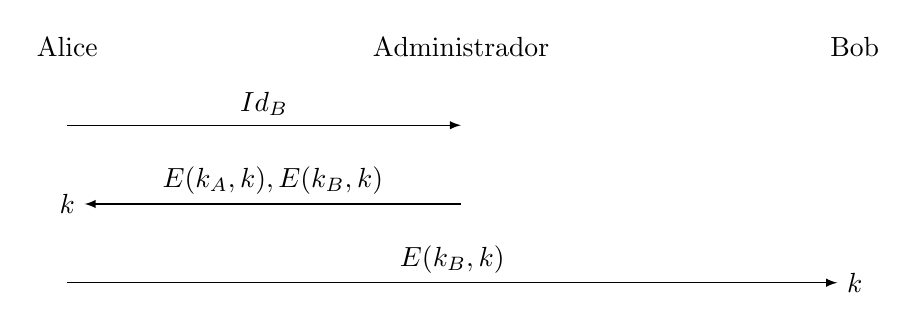
\begin{tikzpicture}[node distance=2cm,auto,>=latex]
\node (alice) at (0, 2){Alice};
\node (bob) at (10, 2) {Bob};
\node (servidor) at (5, 2) {Administrador};

\node (k1) at (0,0) {$k$};
\node (k2) at (10,-1) {$k$};

\path[->] (0,1) edge node[above]{$Id_B$} (5,1);
\path[->] (5,0) edge node[above]{$E(k_A,k), E(k_B,k)$} (k1);
\path[->] (0,-1) edge node[above]{$E(k_B,k)$} (k2);
\end{tikzpicture}
\end{center}

Depois que a comunicação entre Alice e Bob é concluída, ambos devem {\em descartar a chave efêmera} que foi utilizada.
Isso é importante porque essa chave é válida apenas para aquela sessão específica de comunicação.
Se Alice precisar se comunicar novamente com Bob no futuro, ela deverá solicitar ao administrador uma nova chave efêmera.

Uma implementação bastante conhecida desse modelo de Centro de Distribuição de Chaves (KDC) é o {\em protocolo Kerberos}.
Kerberos é amplamente utilizado em ambientes corporativos para gerenciar a autenticação e a segurança de comunicações, seguindo os princípios do KDC.

No entanto, o modelo KDC tem algumas limitações importantes.
Ele pressupõe a existência de um administrador confiável que gerencia todas as chaves permanentes dos usuários.
Além disso, esse modelo possui um problema significativo conhecido como ponto único de falha.
Isso significa que se o servidor do administrador falhar, todas as comunicações seguras entre os usuários ficarão interrompidas.

Portanto, embora o modelo KDC possa funcionar bem em ambientes fechados com uma hierarquia bem definida, ele não é ideal.
Em ambientes abertos e distribuídos, onde não há uma autoridade central confiável ou onde a disponibilidade contínua do servidor não pode ser garantida, esse modelo é inadequado e pode levar a falhas significativas na segurança e na comunicação.

\section{Protocolo de Diffie-Hellman}
\label{sec:diffie-hellman}


Em um ambiente aberto, onde as partes não têm a possibilidade de encontrar um administrador previamente, confiar em uma autoridade central para a distribuição de chaves não é realista.
No entanto, existe uma solução surpreendente:
é possível que as partes troquem chaves diretamente entre si, mesmo utilizando um canal de comunicação inseguro.

O método que apresentaremos nesta seção é conhecido como {\em protocolo de Diffie-Hellman}, que marca o início do paradigma revolucionário da {\em criptografia assimétrica}.
Nos próximos capítulos, exploraremos esse conceito em mais detalhes \cite{Diffie76}.

Informalmente, o protocolo de Diffie-Hellman funciona da seguinte maneira:
Alice e Bob trocam entre si alguns dados públicos.
A partir desses dados, ambos conseguem calcular um valor comum, que pode ser usado como entrada em uma função de derivação de chaves (KDF - Key Derivation Function) para gerar uma chave secreta compartilhada.
O interessante é que, para um observador externo (que chamaremos de Eva), que só teve acesso aos dados públicos trocados, é impossível calcular esse valor comum e, consequentemente, a chave secreta.

Para explicar o protocolo precisamos definir o que são grupos, geradores e grupos cíclicos e precisamos apresentar o {\em problema do logaritmo discreto} cuja dificuldade é condição necessária -- apesar de insuficiente -- para a segurança do protocolo.

Um {\em grupo} é uma estrutura matemática que possui duas partes:
\begin{itemize}
\item Um {\em conjunto} que podemos chamar de $G$.
\item Uma {\em operação} que combina dois elementos desse conjunto e resulta em um terceiro elemento do mesmo conjunto.
  Essa operação pode ser algo como adição, multiplicação, ou outra forma de combinação.
  \end{itemize}

Para que essa estrutura seja considerada um grupo, a operação deve seguir algumas regras específicas:
\begin{itemize}
\item[] {\bf (fecho)} Se você pegar dois elementos de $G$ e usar a operação entre eles, o resultado também deve ser um elemento de $G$.
  Por exemplo, se $G$ for o conjunto dos números inteiros e a operação for a adição, então somar dois números inteiros sempre dará outro número inteiro.
\item[] {\bf (identidade)} Dentro do conjunto $G$, deve existir um elemento especial que não muda o valor de outros elementos quando usado na operação.
  Esse elemento é chamado de {\em identidade}.
  No caso da adição dos números inteiros, esse elemento é o zero, porque somar zero a qualquer número não altera o número.
  No caso da multiplicação o elemento neutro é o um.
\item[] {\bf (inverso)} Para cada elemento em $G$, deve existir outro elemento em $G$ que, quando combinado com ele usando a operação, resulta na identidade.
  Por exemplo, para a adição, o inverso de um número é o seu oposto (como $3$ e $-3$), porque somá-los dá zero.
\item[] {\bf (associatividade)} A forma como os elementos são agrupados na operação não deve alterar o resultado. Isso significa que, ao combinar três ou mais elementos, não importa se você combina os dois primeiros ou os dois últimos primeiro – o resultado será o mesmo.
  Ou seja, $(a + b) + c = a + (b + c)$.
\end{itemize}

Um grupo pode ser finito ou infinite dependendo se o conjunto $G$ tiver um número limitado de elementos ou não.
Quando ele é finito, o número total de elementos em $G$ é chamado de {\em ordem} do grupo.

Além disso, se a operação der o mesmo resultado independentemente da ordem em que você combina os elementos, o grupo é chamado de {\em abeliano} ou {\em comutativo}.

O conjunto dos número inteiros com a operação de adição é um grupo abeliano.
Já o conjunto dos números naturais não é porque nenhum número natural tem inverso aditivo.

O conjunto dos números inteiros com a operação de multiplicação não é um grupo porque, com exceção do $1$, nenhum outro elemento tem inverso multiplicativo.
Já o conjunto dos número racionais sem o $0$ é um grupo.

Vamos apenas apresentar um grupo finito:
\begin{example}
  Se $p$ um número primo, o conjunto $\mathbb{Z}_p^\star = \{ 1, \dots, p-1\}$ que possui $p$ elementos com a operação de multiplicação módulo $p$ é um grupo (Lembre que o módulo o resto da operação por $p$).

    Não é difícil se convencer de que essa estrutura é fechada, associativa e que o $1$ é seu elemento neutro.
    O difícil é motrar que todos elementos possuem inverso.

    Mais para frente vamos tentar provar isso, por hora veja o exemplo do conjunto $\mathbb{Z}_7^\star$.
    Todos seus elementos tem um inverso multiplicativo:
    
    \begin{multicols}{2}
    \begin{itemize}
      \item[] $1^{-1} \equiv 1\ mod\ 7$
      \item[] $2^{-1} \equiv 4\ mod\ 7$
      \item[] $3^{-1} \equiv 5\ mod\ 7$
    \end{itemize}
    \begin{itemize}
      \item[] $4^{-1} \equiv 2\ mod\ 7$
      \item[] $5^{-1} \equiv 3\ mod\ 7$
      \item[] $6^{-1} \equiv 6\ mod\ 7$
    \end{itemize}
  \end{multicols}
\end{example}

Para nossos propósitos, será útil definir como funciona a operação de exponenciação dentro de um grupo.
Se temos um elemento $g$ em um grupo $G$, e um número inteiro positivo $m$, podemos definir a exponenciação de $g$ pelo número $m$ como a operação de combinar $g$ consigo mesmo $m$ vezes (vamos usar o símbolo $circ$ para representar uma operação genérica):

\begin{displaymath}
  g^m := \underbrace{g \circ \dots \circ g}_m
\end{displaymath}


\begin{theorem}[Euller]
\label{theo:gen-euler}
Seja $G$ um grupo abeliano finito de tamanho $m$, então para qualquer elemnto $g$ temos que:

\begin{displaymath}
  g^m = 1
\end{displaymath}
\end{theorem}
\begin{proof}
  Note que se $g \circ g_i = g \circ g_j$ então $g_i = g_j$.
  Assim temos que $\{(g \circ g_1), \dots, (g \circ g_m)\}$ tem todos os elementos de $G$ porque todos eles são distintos e há $m$ elementos.
  Assim temos que:

  \begin{eqnarray*}
    g_1 \circ \dots \circ g_m & = & (g \circ g_1) \circ \dots \circ (g \circ g_m)\\
                              & = & g^m \circ (g_1 \circ \dots \circ g_m)
  \end{eqnarray*}
  Multiplicando ambos os lados pelo inverso de $g_1 \circ \dots \circ g_m$ temos que $g^m = 1$.
\end{proof}

Se pegarmos um elemento específico $g$ de um grupo e começarmos a combiná-lo repetidamente consigo mesmo, vamos gerar uma sequência de novos elementos.
Por exemplo, começamos com o próprio elemento, depois combinamos ele com ele mesmo, depois combinamos o resultado com ele novamente, e assim por diante.
O conjunto de todos os elementos que conseguimos gerar dessa forma é o que chamamos de conjunto dos elementos gerados por aquele elemento específico.

Escrevemos assim o conjunto gerado pelo elemnto $g$:
\begin{displaymath}
  \langle g \rangle := \{g^0, g^1, \dots \}
\end{displaymath}

A {\em ordem} de um elemento é o número de vezes que precisamos combiná-lo consigo mesmo até que ele ``volte'' ao ponto de partida, ou seja, até que o resultado seja o elemento especial do grupo que não muda nada quando combinado com outros (como o 0 na adição ou 1 na multiplicação).

O teorema anterior nos diz que esse número (a ordem) é sempre menor ou igual ao número total de elementos do grupo.
Isso significa que, em um grupo finito, o conjunto dos elementos gerados por qualquer elemento específico também será finito.

Finalmente, um grupo é chamado de {\em cíclico} se existe um elemento especial dentro dele, chamado de {\em gerador}, que, quando combinado repetidamente consigo mesmo, é capaz de gerar todos os elementos do grupo.
Em outras palavras, o conjunto dos elementos gerados por esse gerador é exatamente o grupo inteiro ($\langle g \rangle = G$).

Em um grupo cíclico com gerador $g$, qualquer elemento $h$ dentro desse grupo pode ser obtido ao combinar $g$ consigo mesmo um certo número de vezes $x$.

Esse número $x$ é chamado de logaritmo de $h$ na base $g$.
Ou seja, $log_g(h)$ é o número de vezes precisamos combinar o gerador $g$ consigo mesmo para chegar ao elemento $h$ no grupo.

\begin{example}
Considere o grupo $\mathbb{Z}_7^\star$ com a operação de multiplicação:
\begin{itemize}
\item $\langle 2 \rangle = \{1, 2, 4\}$.
  A ordem de $2$ é $3$ e, portanto, $2$ não é um gerador de $\mathbb{Z}_7^\star$.
  Além disso, neste grupo $log_2(1) = 0$, $log_2(2) = 1$ e $log_2(4) = 2$.
\item $\langle 3 \rangle = \{1, 3, 2, 6, 4, 5\}$.
  A ordem de $3$ é $6$, portanto $3$ é um gerador de $\mathbb{Z}_7^\star$ e o grupo é cíclico.
Além disso, neste grupo $log_3(1) = 0$, $log_3(2) = 2$ e $log_3(3) = 1$, $log_3(4)= 4$, $log_3(5) = 5$ e $log_3(6) = 3$.
\end{itemize}
\end{example}

O {\em protocolo de Diffie-Hellman} permite que duas pessoas, Alice e Bob, compartilhem uma chave secreta para comunicação, mesmo que estejam usando um canal público.
Funciona assim:
\begin{enumerate}
\item  Alice começa criando um grupo cíclico e escolhendo um gerador desse grupo.
  Esse gerador é usado para criar outros elementos no grupo.
\item Alice então escolhe um número secreto, que chamamos de $x$, e usa esse número para calcular um valor $h_A$, combinando o gerador consigo mesmo $x$ vezes.
  Ou seja, $h_A = g^x$.
\item Alice envia para Bob o grupo que ela criou, o gerador, e o valor $h_A$ que ela calculou.
(As vezes $h_A$ é chamado de chave pública de Alice e $x$ sua chave privada).
\item Quando Bob recebe essas informações, ele também escolhe um número secreto, $y$, e usa esse número para calcular um valor $h_B$, combinando o gerador $g$ consigo mesmo $y$ vezes.
  Ou seja, $h_b = g^y$.
\item Agora Bob envia $h_B$ para Alice.
  (As vezes $h_B$ é chamado de chave pública de bob e $y$ sua chave privada).
\item Agora, Alice e Bob podem calcular uma chave secreta que ambos compartilham.
  Alice usa o valor $h_B$ que recebeu de Bob, e eleva-o a $x$ que ela escolheu, para obter a chave $h_B^x = (g^y)^x = g^{xy}$.
  Bob faz a mesma coisa, eleva $h_A$ que recebeu de Alice, e elevá-o ao seu número secreto $y$ para obter $h_A^y = (g^x)^y = g^{xy}$
\end{enumerate}

No final do processo, tanto Alice quanto Bob conseguem calcular o valor $g^{xy}$ que pode ser usado para gerar uma chave (usado como material para a chave).
Alice consegue fazer isso porque ela conhece seu próprio número secreto $x$ e o valor $g^y$ que recebeu de Bob.
Da mesma forma, Bob consegue calcular $g^{xy}$ porque ele conhece seu número secreto $y$ e o valor $g^x$ que recebeu de Alice.

Agora, se alguém estiver espionando a comunicação entre Alice e Bob, essa pessoa (vamos chamá-la de Eva) só terá acesso aos valores $g^x$ e $g^y$.
Para descobrir a chave secreta, Eva precisaria descobrir $x$ a partir de $g^x$ (ou $y$ a partir de $g^y$, que é equivalente).
Isso significa que Eva precisaria resolver o logaritmo discreto — ou seja, encontrar o número $x$ que satisfaz a equação $g^x = h_A$.

Existe uma forma simples de Eva calcular o logaritmo discreto, que é o que chamamos de força bruta.
Para isso ela teria que testar todos os valores possíveis de $x$ até encontrar o correto. Esse tipo de ataque é linear no número de possíveis valores de $x$, mas se $x$ for grande um tipo de ataque como esse é inviável na prática.

Em resumo, o protocolo de Diffie-Hellman é seguro se o problema do logaritmo discreto para o grupo escolhido for difícil.


Você pode estar se perguntando:
``Mas Bob também não teria que tentar todas as possibilidades para calcular \( g^{xy} \)?''
A resposta é {\em não}, e isso é porque Bob pode usar um método muito mais eficiente para fazer essa exponenciação.

Primeiro, vamos entender o método ``ingênuo'' de calcular $g^x$.
A ideia básica é que você pode calcular $g^x$ multiplicando $g$ por ele mesmo $x$ vezes, como mostrado abaixo:

\begin{displaymath}
  g^x = g \circ g^{x-1}
\end{displaymath}

Nesse método, começamos com $g^0 = 1$, já que qualquer número elevado a zero é 1.
Depois, continuamos multiplicando $g$ até chegar a $g^m$.
Esse procedimento pode ser implementado de maneira simples, mas não é muito eficiente, pois leva $m$ passos para completar o cálculo.
O tempo necessário para esse cálculo cresce linearmente com $m$ e exponencialmente com o tamanho de $m$ (lembre que podemos escrever o número $m$ em notação binária usando $log_2(m)$ dígitos), o que significa que o método fica muito lento para números grandes.

No entanto, podemos fazer isso de maneira muito mais rápida usando um truque inteligente chamado \textit{exponenciação rápida}.
Em vez de calcular $g^m$ multiplicando $g$ repetidamente, podemos dividir o problema em partes menores e resolver cada parte de forma mais eficiente:

\begin{displaymath}
  g^m = \left\{
    \begin{array}{lcl}
      \text{Se } m \text{ é par:} & g^{m/2} \circ g^{m/2} \\
      \text{Se } m \text{ é ímpar:} & g^{\lfloor m/2 \rfloor} \circ g^{\lfloor m/2 \rfloor} \circ g \\
    \end{array}
  \right.
\end{displaymath}

Em vez de precisar de $x$ passos, agora precisamos de apenas $\log_2(x)$ passos, o que é muito menor.
Assim, o tempo necessário para calcular $g^m$ cresce linearmente com o tamanho do número $m$, o que torna esse método extremamente eficiente, mesmo para números grandes.

Por exemplo, se quisermos calcular $2^{10}$ usando a exponenciação rápida, o processo seria o seguinte:

\begin{displaymath}
  \begin{array}{ll}
    \text{FastExp}(2, 10) = x \cdot x = 2^{10} & x = \text{FastExp}(2, 5) = 2^5 \\
    \text{FastExp}(2, 5)  = x \cdot x \cdot 2 = 2^5 & x = \text{FastExp}(2, 2) = 2^2\\
    \text{FastExp}(2, 2)  = x \cdot x = 2^2 & x = \text{FastExp}(2, 1) = 2\\
    \text{FastExp}(2, 1)  = x \cdot x \cdot 2 = 2 & x = \text{FastExp}(2, 0) = 1\\
    \text{FastExp}(2, 0)  = 1 \\
  \end{array}
\end{displaymath}

Com esse método, calculamos $2^{10}$ em muito menos passos do que se usássemos a abordagem ingênua.

A dificuldade em resolver o problema do logaritmo discreto é uma condição necessária, mas não suficiente por si só, para garantir a segurança do protocolo de Diffie-Hellman.
Existem certas estruturas matemáticas que são bem adequadas para criar grupos cíclicos onde o problema do logaritmo discreto é considerado difícil de resolver.
Duas das mais utilizadas na prática são os {\em resíduos quadráticos em grupos de tamanho primo} e as {\em curvas elípticas} (discutidas no Apêndice \ref{cha:ciclicos}).

Se o problema do logaritmo discreto fosse fácil, uma espiã como Eva poderia encontrar os valores secretos $x$ e $y$ a partir de $g^x$ e $g^y$, descobrindo assim o valor de $g^{xy}$.
No entanto, em um sistema seguro, o melhor que Eva poderia fazer seria tentar todos os possíveis valores de $x$ ou $y$ até encontrar o correto, o que é impraticável se o grupo for grande o suficiente.
Portanto, ao escolher grupos de ordem suficientemente grande, essa tarefa se torna computacionalmente inviável.

Uma vez que Alice e Bob possuem o mesmo valor secreto $g^{xy}$, eles podem usá-lo para alimentar uma função de derivação de chave (KDF), gerando assim as chaves necessárias para um sistema de criptografia simétrico.

Na teoria, assumimos que o grupo e o gerador são criados cada vez que Alice e Bob decidem se comunicar.
Na prática, porém, é mais comum que esses parâmetros sejam definidos pelo protocolo e reutilizados em todas as comunicações.
Isso não afeta a segurança do sistema.

Caso o problema do logaritmo discreto não seja difícil, Eva seria capaz de produzir $x$ e $y$ a partir de $g^x$ e $g^y$ e descobrir o valor de $g^{xy}$.
Se o sistema for seguro, porém, o melhor que Eva pode fazer é tentar todos os valores de $\mathbb{Z}_n$ até encontrar $x$ ou $y$.
Escolhendo grupos de ordem suficientemente grande, essa tarefa é computacionalmente inviável.
Uma vez que as partes possuem o mesmo valor secreto, elas podem utilizá-lo para alimentar um KDF e gerar chaves para um sistema de criptografia simétrico.

No modelo, assumimos que o grupo e o gerador são criados sempre que as partes decidem se comunicar.
Na prática o mais comum é que esses parâmetros sejam definidos pelo protocolo e reutilizados em todas as comunicações.
Isso não deve afetar de nenhuma forma na segurança do sistema.

Embora o Diffie-Hellman permita a criação de uma chave secreta sem a necessidade de uma reunião física ou uma autoridade central confiável, ele não garante a autenticidade das partes envolvidas na comunicação.
Isso significa que o protocolo é vulnerável a um tipo de ataque conhecido como ``Man in the Middle'' (MitM).
Voltaremos a isso no Capítlo \ref{cha:assinaturas-digitais}.

\section{Exercícios}
%\label{sec:exercicios}

\begin{exercicio}
  Mostre que se $n|a$ e $n|b$ então para quaisquer $r$ e $s$ temos que $n|(a \cdot r + b \cdot s)$.
\end{exercicio}

\begin{exercicio}
\label{ex:grupo}
  Considere a estrutura $\langle \mathbb{Z}_{12}, \cdot \rangle$ em que a multiplicação é calculada módulo 12.
Mostre que $6$ não possui inverso nesta estrutura e, portanto, ela não é um grupo.
\end{exercicio}

\begin{exercicio}
  Considere as estruturas $\langle \mathbb{Z}_n, + \rangle$ formadas pelo conjunto $\mathbb{Z}_n := \{0, \dots, n-1\}$ e a operação de soma ($+$) módulo $n$.
  Mostre essa estrutura é um grupo cíclico para qualquer valor de $n \geq 1$ e que o número $1$ é sempre um gerador nesses grupos. (Dica: Você precisa mostrar que a operação satisfaz fecho, associatividade, possui elemento neutro e inverso. Depois você deve mostrar que o elemento $1$ gera todos os elementos do grupo.)

  Por que o grupo $\langle \mathbb{Z}_n, +\rangle$ não é um bom candidato para ser usado no protocolo de Diffie-Hellmann.
\end{exercicio}

\begin{exercicio}
  Descreva um ataque força-bruta contra o protocolo de Diffie-Hellman.
  Em termos assintóticos em relação ao tamanho da entrada, qual é o consumo de tempo deste ataque?
\end{exercicio}
